\chapter{Implemented Modules}

In this chapter, the technical goals of the project are introduced. Each developed module will be explained as well as it's requirements and it's specification details. For each module, it will be explored:

\begin{itemize}
  \item The technical goals
  \item The problem to which the module provides a solution
  \item Some of it's properties (reusability, scalability \dots)
  \item Integration with the current version of Aerostack
\end{itemize}

\section{Technical Goals}

  % ToDo := introduce the goals: problem and solution each module solves
  In order for the Aerostack framework to localize with a different technique rather than visual markers a lidar sensor will be used. In this case, the \textit{Hokuyo Eye} range sensor will be used, which is the \textit{defacto} range sensor in this context. Also, the low level implentation provides a nice ros API that can be used to fetch data. To wrap all this functionallity we propose the implementation of a new high level behavior that coordinates all the framework with the lidar interface, providing a high level, standarized API for lidar-based localization.

  As of the current version of Aerostack, navigation is done with a 2D probabilistic roadmap planner, the input for the planner is a predefined map, done by hand in the Graphical User Interface that Aerostack provides. This is a static map and goes against the nature of the any dynamically acquired mapping signal. To tackle this problem a new navigation behavior is proposed. This behavior will abstract the planner used for each localization mode, providing a high level standarized API that can be used independently of the localization technique, replacing the old one.

\section{Specification}

  Each implemented module should follow the specification imposed by the Aerostack framework. In Aerostack there are different types of processes providing structure and added functionallity. When a new process is created it should be decided whether to implement it as a plain, simple ros node, a robot process or a behavior process. Their differences are as follows:

  \begin{itemize}
    \item ROS Node: This is the standard way of adding modules in a ROS oriented architecture. A ros node is simply a process programmed in any of the programming languages supported by ros (C, C++, Python \dots) that implements a task and is interfaced through the ros master server with named topics, services or both. A ros node can subscribe or publish topics and optionally, provide services, as many topics or services as it wants. These topics and services are nothing more than binded ports to the ROS master server, that works over TCP (normally) or UDP to distribute traffic. This is the implementation to follow when adding very low level modules, like platform drivers.
    \item Robot Process: A Robot Process is an abstraction provided by Aerostack, it serves mainly as a standarization layer, providing an interface for the rest of the architecture to be used. It provides three services to manage the process, one for stopping it, one for starting it and another one to check whether it is running or not, aditionally it emits an alive signal every second or an error signal when the thread crashes. It runs the inheritors' code inside a separate thread in order to monitor it. When adding a module that abstracts some low level APIs, like a visual marker processor, this is the class to inherit from.
    \item Behavior Process: This is the highest level of the hierarchy, inside the Aerostack framework there exists a process that coordinates all the behaviors, to do so, every behavior exposes an interface similar to the Robot Process and a configuration file that especifies the mid and low level processes the behavior depends upon (it's capabilities and incompabilities), amongst other parameters, in this sense, the behavior that provides localization based on visual markers depends on the visual marker processor to work. Formally, a behavior is just a high level process that monitors an algorithm: it runs the algorithm in a separate thread and emits the state and error signals, listening to \textit{start/stop} events and acting accordingly over the algorithm. When adding a high level functionallity, this is the class that should be inherited.
  \end{itemize}

  In a similar fashion to the visual marker localization behavior, the lidar localization behavior proposed will require three more processes: the slam process, an ekf that combines various signals and a localization technique selector, this is explained in detail in the corresponding behavior section (sect. \ref{ch_4:sect:behav_slam}).

  The case of the navigation behavior is more complicated as it will need more modules to work correctly and will make use of other behaviors [\textbf{ToDo := Tell a little what modules does the navigator requires}]

  % ToDo =: Tell about the navigator.

\section{Integration} \label{ch_4:sect:integration}

  % ToDo := How does the module integrates with the current state of Aerostack
  To integrate each behavior, we will follow a bottom up procedure. This way, we will ensure that the processes the behavior depends on are working correctly inside the Aerostack and the error doesn't get masked with the behavior integration.

  When integrating a new behavior some steps should be followed:
  \begin{itemize}
    \item Add the necessary mid and low level processes to the Aerostack and ensure they can be started automatically.
    \item Add the technical specification of the behavior to the behavior catalog. These are the capabilities and incompabilities of the behavior and should include the mid and low level processes previously mentioned so that they can be started automatically. In this step, the behaviors that are incompatible with the new one should be identified.
    \item Add the implementation of the behavior and test it with the Aerostack to ensure it can be started and that no incompatibilities arise.
  \end{itemize}

  The lidar-based localization behavior will provide a new localization mode, so it is reasonable to mark the rest localization behaviors as incompatible, also, a new localization method selector process will be added, this will ensure that when various localization techniques are to be used in the same mission, they can be easily toggled on and off. This will be detailed in the corresponding behavior section \ref{ch_4:sect:behav_slam}.

  In the case of the navigation behavior, the rest of the navigation behaviors will be marked as incompatible, but as this behavior is intended to replace the old one, no selector will be provided. Instead, this behavior will choose the data sources and plan with that data, providing an abstraction over the method used for localization and mapping.

\section{Behavior Self Localize and Map by Lidar} \label{ch_4:sect:behav_slam}

  The lidar range sensor outputs raytraces reflected over the near objects, in a way, it resembles a sonar sensor (that's way it's called lidar). Each raytrace, measures the distance from a concrete angle to a point at a certain distance, these measures then have to be converted in some way that can be used to map the environment and use this mapped environment to localize inside it (see section \ref{ch_3:sect:localization:slam} for an in-depth explanation of SLAM). Refer to figure \ref{ch_4:fig:behav_slam} for a visual representation of the behavior and it's subprocesses.

  We will use a ros module implemented by the same laboratory as the SLAM node \cite{hector_slam}: hector mapping. It will output the estimated localization along with the mapped environment. This localization will be merged with the measures from the rest of the sensors (namely odometry, IMU \dots) using an extended kalman filter (see section \ref{ch_3:sect:localization:ekf}) to output a robust estimate of the robot's position inside the mapped world. 

  The process in charge of the EKF is called \textit{droneRobotLocalization} and inherits from \textit{Robot Process} class. It will listen for updates on the robot's pose (\textit{hector\_pose}) and the both the IMU and the odometry topics and output the estimated pose.

  \begin{figure}[h] 
    \centering
    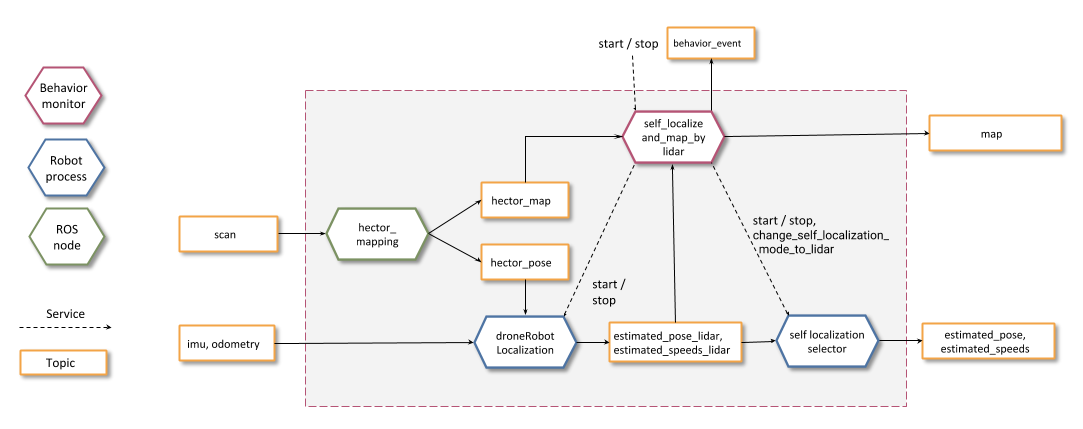
\includegraphics[width=\textwidth]{./Figures/BehaviorSlamArquitecture.png}
    \caption{Behavior self localize and map by lidar architecture. \textit{Hector mapping} is the SLAM module from \cite{hector_slam}. \textit{Drone Robot Localization} does the EKF. \textit{Self Localization Selector} gives the localization based on the selected technique.}
    \label{ch_4:fig:behav_slam}
  \end{figure}

  The estimated pose is then fed to the selector, which will toggle the localization technique. This implementation opens the door to new localization behaviors, a GPS based one for instance and also makes compatible the previous ones (visual markers based). It is easy to think of an scenario that requires both indoor and outdoor localization, in such a mission, the localization technique in use should be toggled in order for the navigator to work properly. As can be seen in Fig. \ref{ch_4:fig:behav_slam}, this is a \textit{Robot Process} with an added service to change the localization technique used.

  Bellow there is a list of the inputs and outputs of this behavior:

  % ToDo := Check this out with Martin
  [\textbf{ToDo := Set this up as a table??}]
  \begin{itemize}
  \item scan: This is the output of the lidar node, it is directly fed into the \textit{hector mapping} node
  \item imu: This topic contains the measures from the \textit{inertial measurement unit}
  \item odometry: This is a general topic with the measures from odometry
  \item map: This is the map as processed by the \textit{hector mapping} node
  \item estimated\_speed\_lidar: This is the estimated speed from the whole behavior process, fed to the selector
  \item estimated\_pose\_lidar: This is the estimated pose from the whole behavior process, fed to the selector
\end{itemize}

  This behavior monitors the correct working of the algorithm (\textit{hector mapping}) by listening on the \textit{map} topic, when it outputs strange or simply wrong data, an error is emitted.

  In the configuration file of this behavior the localization by visual markers behavior will appear as incompatible. As for the capabilities, all of \textit{hector mapping}, \textit{drone robot localization} and \textit{self localization selector} will figurate as capabilities, indicating that those processes should be started before this behavior.

\section{Behavior Navigation Interface}

This behavior should provide an API to do navigation tasks. It should be able to generate obstacle-free trajectories  to any given point (when there exists one) and be able to move the robot along those trajectories.

\pagebreak

The identified tasks for this behavior are as follows:

\begin{enumerate}
  \item Given a point (or goal), execute the necessary motions to get the robot to that goal.
  \item Given a path, execute the necessary motions to follow it until the path is finished.
  \item Given a point (or goal), generate an obstacle-free path from the current robot's position to that goal.
\end{enumerate}

This tasks can be directly mapped with processes. However, we will implement them as separate behaviors to provide more modularity and reusability. 

As of the current version of Aerostack, there exists a behavior that executes the motion of going to a given point in the 2D map representation used by Aerostack. However, this behavior is not general enough to use a different map representation, so we will implement a new one capable of executing the motion in the new map format: occupancy grids (which is the format used in \textit{hector mapping}).

The task of following a path can also be broken down to generate a series of points along that path and following each point. Following points blindly can be dangerous in environments whith moving obstacles, therefore a new behavior for this functionallity will be provided. This new behavior will receive a path, chop it in various points and start following them, testing before each motion if the path is obstacle-free. To do so, it will make use of the trajectory generator.

With all this information, the \textit{behavior navigation interface} can be defined as the process in charge of coordinating all these new behaviors, it will receive a point and work in tandem with the other three behaviors to manage to go to that point without colliding with any obstacle.

The proposed names for each behavior are: \textit{behavior go to point in occupancy grid}, \textit{behavior follow path in occupancy grid}, \textit{behavior generate path in occupancy grid}. Figure \textbf{ToDo := Generate figure} ilustrates the architecture followed for all these behaviors and the more general \textit{behavior navigation interface}

% ToDo := Add nav behavior figure.

In order to integrate this new behaviors with the current version of the Aerostack, the following topics will be created:

\textbf{TODO := Table with all the generated topics and it's description}

The following subsubsections explain each behavior in more detail.

\subsection{Behavior Go to Point in Occupancy Grid}

In order to move the robot from one point to another, this behavior will communicate the controller, providing it with the desired point. The controller will translate this point in the necessary motions and move the robot. Furthermore a \textit{cancel motion} service will be provided to cancel the motion in course, giving grainer control to the navigation interface.

\subsection{Behavior Follow Path in Occupancy Grid}

This behavior will work in tandem with the go to point process, it will receive a path as a list of points and ask the \textit{behavior go to point in occupancy grid} for each each point. Additionally, it will include the \textit{cancel motion} service too.

\subsection{Behavior Generate Path in Occupancy Grid}

In this case we will employ a special planner provided as a ros package called \textit{move base}, which is specially crafted for lidar interfaces. It accepts an occupancy grid map and the raytraces from the lidar and implements the planning algorithm. \textbf{TODO := Talk more over the move algorithm, explain the behavior monitoring.}

% ToDo := Finish redacting this behavior

\begin{comment}
  \begin{itemize}
  \end{itemize}
\end{comment}
